%%%%%%%%%%%%%%%%%%%%%%%%%%%%%%%%%%%%%
\begin{frame} [plain]
    \frametitle{}
    \Background[1] 
    \begin{center}
    { {\huge 第一章:绪论 }}
    \end{center}  
    \addtocounter{framenumber}{-1}   
\end{frame}
%%%%%%%%%%%%%%%%%%%%%%%%%%%%%%%%%%

\section{1.课程简介}

\begin{frame}
    \frametitle{课程目标}
        \begin{enumerate}
            \Item Learn the formal theory of Quantum Mechanics
            \IItem How physical systems are described in Quantum Mechanics.
            \Item How to solve problems in Quantum Mechanics.
        \end{enumerate}
\end{frame}
\begin{frame} 
    \frametitle{分数构成}
        \begin{enumerate}
            \Item Normal results 20\%
            \Item Midterm examination results 20\%
            \Item Final examination results 60\%
        \end{enumerate}
\end{frame}

\begin{frame} 
    \frametitle{教学效果}
    \centering
    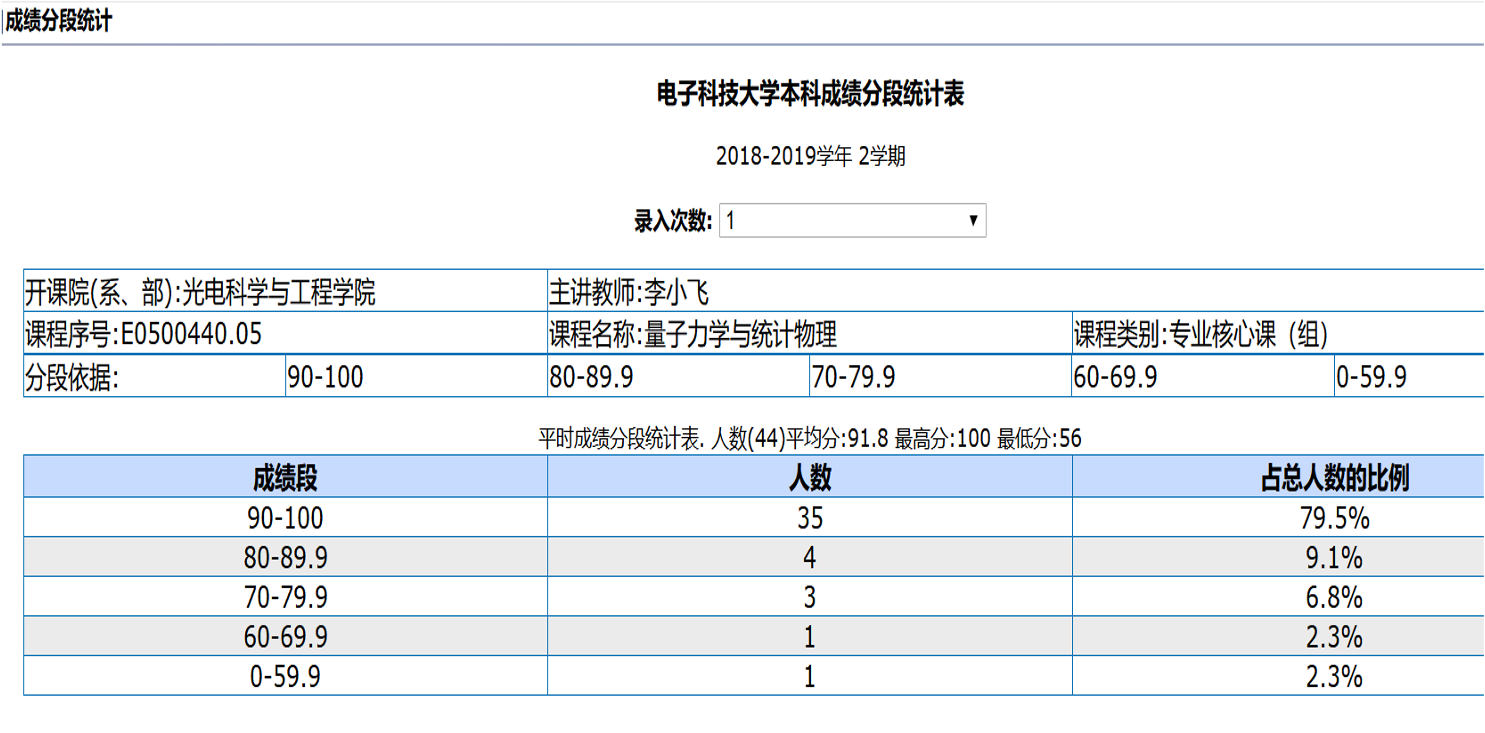
\includegraphics[width=1.0\textwidth,height=5.0cm]{figs/exam1.png}
\end{frame}

\begin{frame}
    \frametitle{参考书目}
        \begin{itemize}
            \Item 《量子力学》卷I,II, 曾谨言, 科学出版社, 2008           
            \Item Principles of quantum mechanics, shankar
            \Item Modern quantum mechanics, shankar
            \Item Lectures on quantum mechanics, weinberg
            \Item Principles of quantum mechanics, Dirac
        \end{itemize}
\end{frame}

\begin{frame}
    \begin{tcolorbox4}[三条军规]    
        \begin{enumerate}
            \Item Objects are wave-particles and can be in states of superposition
            \Item Rule 1 holds as long as you don't measure
            \Item Measurement gives random results
        \end{enumerate}
    \end{tcolorbox4} 
\end{frame}

\section{2.能量子假说}

\subsection{伟大成就}

\begin{frame}[t]
    \frametitle{经典物理伟大成就}
    \begin{tcolorbox3}
    [Great successes in Classical Physics]
        \begin{enumerate}
            \Item Newtonian mechanics
            \Item Maxwell's electromagnetism
            \Item Thermodynamic laws
        \end{enumerate}
    \end{tcolorbox3}  
    \begin{quotation}
        "There is nothing new to be discovered in physics now. All that remains is 
        more and more precise measurements"   \\
        \rightline{$\cdots$ Lord Kelvin (1900)\hspace{3em}}
    \end{quotation}
\end{frame}

\begin{frame}
    \frametitle{}
    \begin{quotation}
        "But the beauty and clearness ... is obscured by two small puzzling clouds \faCloud "  \\
        \rightline{$\cdots$ Lord Kelvin (1900.4)\hspace{3em}}   
    \end{quotation}
    ~~ \vspace{0.3em}
    \begin{tcolorbox4}[两朵乌云]    
        \begin{enumerate}
        \Item Michelson-Morley experiment
        \Item Black body radiation
        \end{enumerate}
    \end{tcolorbox4} 
\end{frame}

\begin{frame}
    \frametitle{迈克尔逊-莫雷实验}
    \begin{center}
    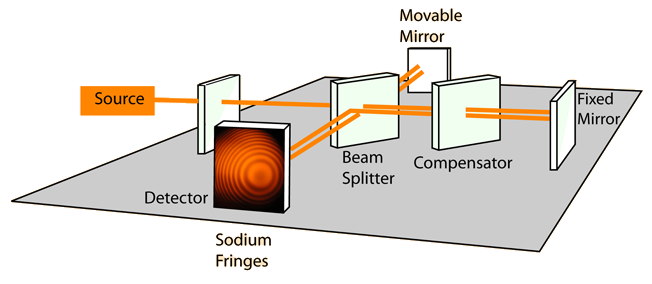
\includegraphics[width=0.8\textwidth]{figs/michel.png}
    \end{center}
There is no displacement of the interference bands. \dots 
the Stationary Ether is thus shown to be incorrect
\end{frame}

\begin{frame}
    The theory of relativity is established 
    \begin{center}
        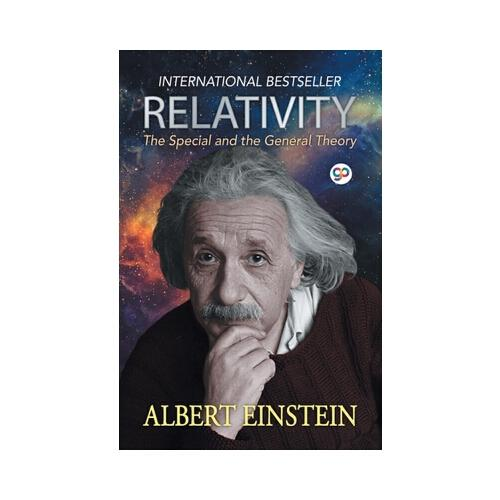
\includegraphics[width=0.4\textwidth]{figs/relativity.jpg}
    \end{center}   
    Greatly changed our view of time and space. Mainly useful in two aspects: high-speed motion, and strong gravitational field. 
\end{frame}

\begin{frame}
    \frametitle{黑体辐射实验}
    \begin{center}
    \includegraphics[width=0.7\textwidth]{figs/2021-12-01-23-47-27.png}
    \end{center}
    No mathematical function to describe the curves exactly 
\end{frame}
\begin{frame}
    Quantum mechanics is established  
    \begin{center}
        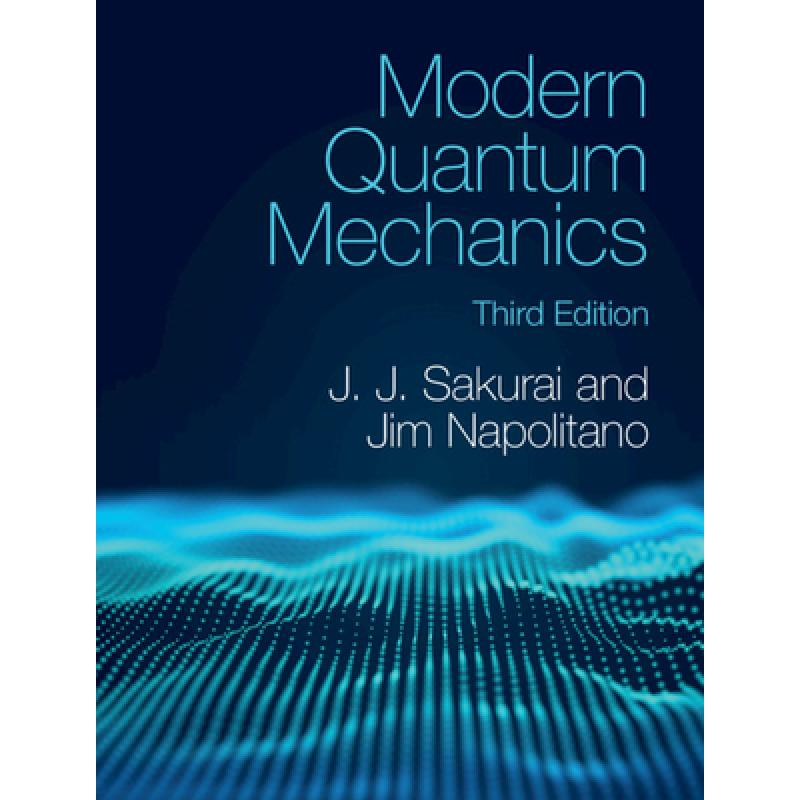
\includegraphics[width=0.45\textwidth]{figs/mqm.jpg}
    \end{center}   
    It is a theory about matter.
\end{frame}

\begin{frame}
    \frametitle{现代科学基石}
    \begin{center}
        \includegraphics[width=0.75\textwidth]{figs/stone.png}
    \end{center}   
\end{frame}

%%%%%%%%%%%%%%%%%%%%%%%%%%%%%%%%%%%%
\subsection{普朗克公式}
%%%%%%%%%%%%%%%%%%%%%%%%%%%%%%%%%%%%

\begin{frame}
    \frametitle{Black body radiation}
    \begin{definition}[Black body: ]
    \hspace{2em}absorb all electromagnetic waves in any temperature
    \end{definition}
    \begin{center}
        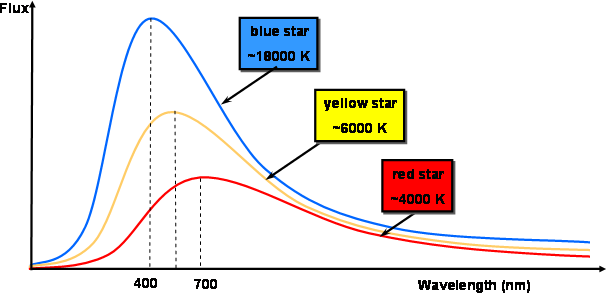
\includegraphics[width=0.55\textwidth]{figs/blackbody_radn_curves.png}
    \end{center}
    \textbf{\color{deepred} Most interestingly}, what is the mathematical function that describes all of these curves?
\end{frame}

\begin{frame}
    \frametitle{三个经验公式}
    \begin{center}
        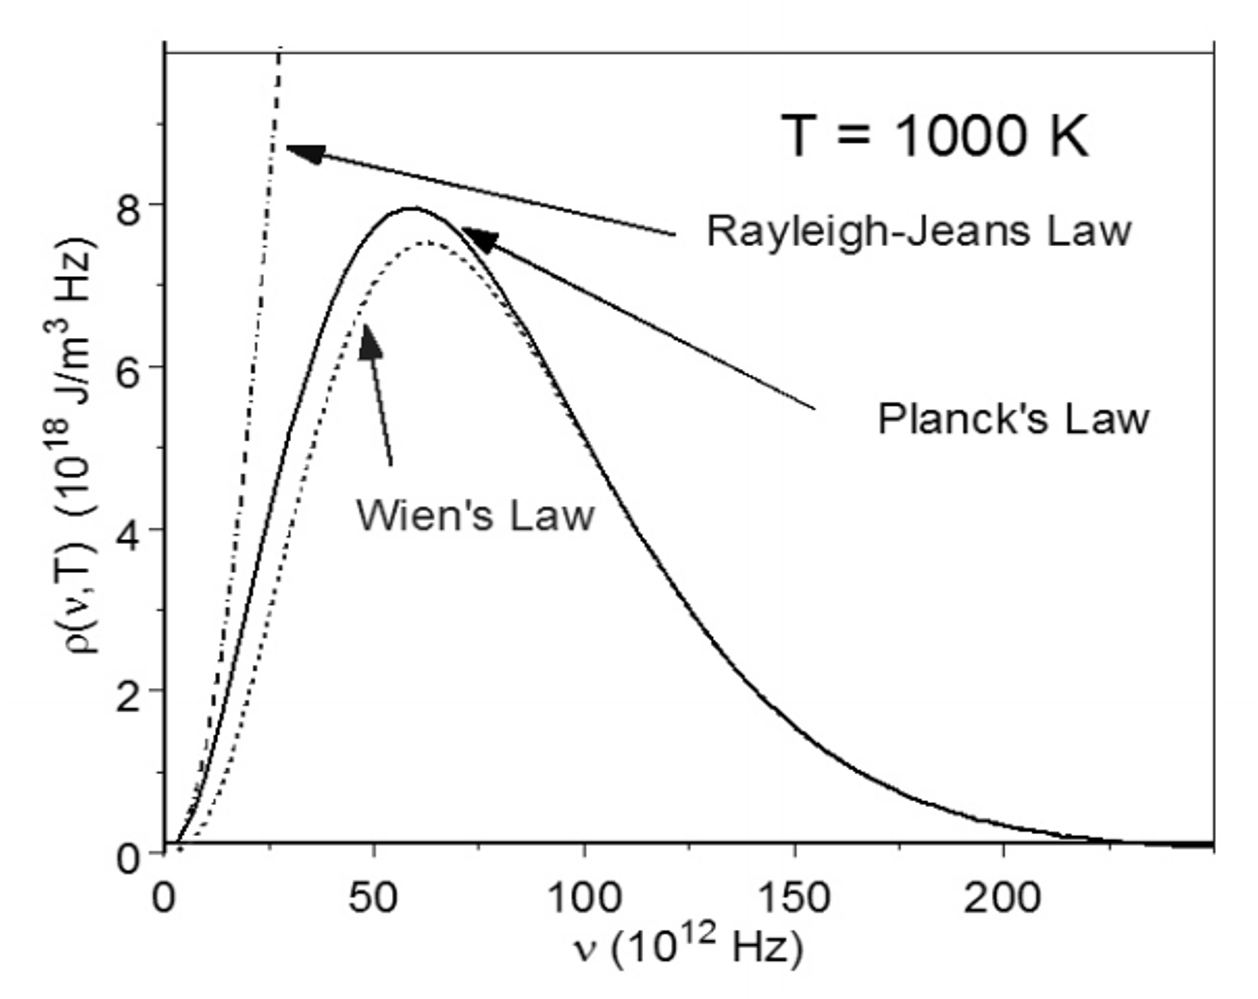
\includegraphics[width=0.7\textwidth]{figs/threelaws.png}
    \end{center}
\end{frame}

\begin{frame} [t]
    \frametitle{维恩公式}
    \begin{equation*}
        \rho(\nu) d \nu=c_{1} \nu^{3} e^{-c_{2} \nu / T} d \nu 
    \end{equation*}
    Derived from electromagnetism (1893), but described well only in high frequency region.\\ 
    {\color{deepred} Nobel Prize in physics(1911)}\\
\end{frame}

\begin{frame}[t]
    \frametitle{瑞-金公式}
    \begin{equation*}
        \rho(\nu, T) d \nu=\frac{8 \pi}{c^{3}} \nu^{2} k T d \nu 
    \end{equation*}
    Derived from thermodynamics (1900), but described well only in low frequency region.\\ 
   {\color{deepred} Nobel Prize in physics(1904)}\\ \vspace{0.3em}
   {\color{deepblue} {\Bullet} Ultraviolet Catastrophe:} 
    \begin{equation*}
         \int_0 ^\infty \frac{8 \pi}{c^{3}} \nu^{2} k T d \nu \to \infty 
    \end{equation*}
\end{frame}

\begin{frame}
    \frametitle{普朗克公式}
    On 1900-10-19, at the German Physical Society, 
    Max Planck presented a resolution to {\color{deepblue} Ultraviolet Catastrophe} 
    \begin{equation}
        \boxed{\rho(\nu, T) d \nu=\frac{8 \pi}{c^{3}} \frac{h \nu^{3}}{e^{h \nu / K T}-1} d \nu}
    \end{equation}
    Obtained from experimental data via interpolation technique, described well in whole region \\
    {\color{deepred} Nobel Prize in physics(1918)}\\
\end{frame}

\begin{frame}
    \centering
    \begin{tcbb}[0.7]{Problems}{
        How to derive the formula from existing theory.}
    \end{tcbb}
\end{frame}

\begin{frame}
    \begin{tcolorbox2}{Solution}
        On 1900-12-14, Planck gives out his solution based on the Energy Quantum Hypothesis  
    \end{tcolorbox2}
\end{frame}

%%%%%%%%%%%%%%%%%%%%%%%%%%%%%%%%%%%%
\subsection{能量子假说}
%%%%%%%%%%%%%%%%%%%%%%%%%%%%%%%%%%%%
\begin{frame}{能量子假说}
    \begin{tcolorbox4}[Energy quantum hypothesis]
    Assuming the oscillators of the cavity could only radiate at a discrete amounts of energy
    \begin{equation}
        E=n\varepsilon
    \end{equation}
    where, the $\varepsilon$ is the unit of the energy (quanta) determined by the oscillator' frequency 
    \begin{equation}
        \varepsilon=h\nu
    \end{equation}
    and the $h=6.6260693(11)\times10^{-34} J\cdot s,\quad (\hbar=\frac{h}{2\pi} \approx 6.58\times 10^{-16} eV\cdot s )$ is the Planck constant. 
    \end{tcolorbox4}
\end{frame}

\begin{frame} {推导公式}
    Based on Boltzmann distribution law,
    \begin{equation*}
        \frac{N_{i}}{N}=\frac{\exp \left(-\frac{E_{i}}{k T}\right)}{\sum_{i} \exp \left(\frac{-E_{i}}{k T}\right)}
    \end{equation*}
    {\Bullet} when the energy is continuous,the distribution between $E - dE$ should be 
    \begin{equation*}
        \frac{e^{-E / k T}}{\int\limits_{0}^{\infty} e^{-E / k T} d E}
    \end{equation*}  
    the average energy 
    \begin{equation*}
        <E>=\int\limits_{0}^{\infty} E \frac{e^{-E / k T}}{\int\limits_{0}^{\infty} e^{-E / k T} d E} d E
    \end{equation*}
\end{frame}

\begin{frame}
    \begin{equation*}
        \begin{split}
            <E> &= -kT \frac{Ee^{-E / k T}\vert_0 ^\infty-\int\limits_{0}^{\infty} e^{-E / k T} d E } {\int\limits_{0}^{\infty} e^{-E / k T} d E }\\  
                &= kT
        \end{split}  
    \end{equation*} 
    {\Bullet} when the energy is discrete,the distribution should be   
    \begin{equation*}
        \frac{e^{-E / k T}}{\int\limits_{0}^{\infty} e^{-E / k T} d E} 
        \to \frac{e^{-E / k T}}{\sum\limits_{0}^{\infty} e^{-E / k T}} 
        \to \frac{e^{-nh\nu / k T}}{\sum\limits_{0}^{\infty} e^{-nhv / k T}} 
    \end{equation*}    
\end{frame}

\begin{frame}
    the average energy 
    \begin{equation*}
        \begin{split}
            <E> &= \sum\limits_{0}^{\infty} nh\nu\frac{e^{-nh\nu / k T}}{\sum\limits_{0}^{\infty} e^{-nh\nu / k T}} \\
            &= -h\nu \frac{d}{dx} \frac{n e^{-nx}}{\sum\limits_{0}^{\infty} e^{-nx}} \\
            &= \frac{h\nu}{e^{h\nu/kT}-1} 
        \end{split} 
    \end{equation*}
    We get
    \begin{equation*}
        \text{(continuous)} \quad k T \rightarrow \frac{h \nu}{e^{ h \nu / k T}-1} \quad \text{(discrete)} 
    \end{equation*}
\end{frame}

\begin{frame}
    In Rayleigh-Jeans formula
    \begin{equation*}
        \rho(\nu, T) d \nu=\frac{8 \pi}{c^{3}} \nu^{2} k T d \nu 
    \end{equation*}
    the item $kT$ should be replaced by $\dfrac{h \nu}{e^{ h \nu / k T}-1}$
    \begin{equation*}
        \rho(\nu, T) d \nu=\frac{8 \pi}{c^{3}} \frac{h \nu^{3}}{e^{h \nu / K T}-1} d \nu
    \end{equation*}
    It is the Planck's formula exactly 
\end{frame}

\begin{frame}
    \begin{tcolorbox4}[Revolutionary Significance]
        Planck's Energy Quantum Hypothesis broke through the constraints of classical physics and 
        opened the door of quantum mechanics 
    \end{tcolorbox4}
\end{frame}

\begin{frame}
    \frametitle{}
    \centering
    \tcbb[0.68]{一只会下金蛋的鹅}
    {
    历史上,普朗克,德拜,艾伦菲斯特,劳厄,洛伦兹,庞加莱,泡利,玻色,爱因斯坦等从多角度推导过普朗克公式,每一次推导都给物理学带来了新的知识内容 
    }

 《黑体辐射公式的多种推导及其在近代物理构建中的意义》- 返朴|曹则贤
\end{frame}

%\begin{frame}
%    \begin{tcolorbox}[colback=yellow!10,colframe=red!75!black,title=THE END]
%    In 1927, Dirac got the Planck's formula from Quantum Mechanism.  
%    \end{tcolorbox}
%\end{frame}

\begin{frame}
    \frametitle{}
    \begin{tcolorbox3}[学术讨论]
        普朗克黑体辐射公式重要,还是能量量子化观念重要?\\
        能量量子化只是一种数学处理工具?
    \end{tcolorbox3}
\end{frame}

%%%%%%%%%%%%%%%%%%%%%%%%%%%%%%%%%%%%%%%%%%%%%%%%%%%%%%%%%%%%%%%%%%%
\begin{frame}
    \frametitle{作业}
   \begin{enumerate}
       \item Planck's Energy Quantum Hypothesis
       \item What's the quanta
       \item Deriving the Rayleigh-Jeans formula and Wien's formula from Planck's formula
   \end{enumerate}
\end{frame}
%%%%%%%%%%%%%%%%%%%%%%%%%%%%%%%%%%%%%%%%%%%%%%%%%%%%%%%%%%%%%%%%%%%

\section{3.波粒二象性}      

\begin{frame}
    \frametitle{}
    \begin{tcolorbox3}[前情回顾]
        Assuming the oscillators can radiate at a discrete amounts of energy
        \[    E=n\varepsilon, \qquad (n=1,2,3,\cdots) \]
        and the unit of the energy is determined by the oscillator' frequency
        \[   \varepsilon=h\nu  \]
        one can derive the framula:
        \[ \rho(\nu, T) d \nu=\frac{8 \pi}{c^{3}} \frac{h \nu^{3} }{e^{h \nu / K T}-1} d \nu \]
    \end{tcolorbox3}
\end{frame}

\begin{frame}
    \frametitle{粒-波的不可调和性}
	\begin{columns}
		\begin{column}[t]{0.46\linewidth}
			粒子性
			\begin{itemize}
				\Item  确定的位置、能量、动量等
				\Item  两个粒子不能同时占据同一位置
				\Item  同一粒子也不能同时占据多个位置
				\Item  碰撞现象
			\end{itemize}
		\end{column}
		\begin{column}[t]{0.46\linewidth}
			波动性
			\vspace{1ex}
			\begin{itemize}
				\Item  确定的波长、振幅、相位等
				\Item  可以同时出现在同一位置
				\Item  可以同时占据多个位置
				\Item  衍射、干涉,无碰撞
			\end{itemize}
		\end{column}
	\end{columns}
\end{frame}

\begin{frame} 
    人们通过上述特性进行判定\\
    \begin{itemize}
        \Item  一个物体要么是粒子,要么是波
        \Item  这个方法一直是有效
        \Item  直到遇到**光** 
    \end{itemize}   
    \begin{figure}
        \centering
        \subfigure[]{\includegraphics[width=7.4cm]{figs/2021-12-02-15-26-40.png}}
        \subfigure[]{
\includegraphics[width=4.5cm]{figs/2021-12-06-11-44-50.png}}
        %\caption{} %图片标题
        %\label{fig:1}  
    \end{figure} 
    \setcounter{subfigure}{0}
\end{frame}

\begin{frame}
	\begin{columns}
		\begin{column}[t]{0.46\linewidth}
            水波
            \begin{center}
                \includegraphics[width=2.5in,height=2.5in]{figs/2021-12-02-15-46-16.png}
            \end{center}
		\end{column}
		\begin{column}[t]{0.46\linewidth}
            光波
            \begin{center}
                \includegraphics[width=2.5in,height=2.5in]{figs/2021-12-02-15-49-36.png}
            \end{center}
		\end{column}
	\end{columns}
\end{frame}

\begin{frame} {光的波动说}
    \begin{center}
        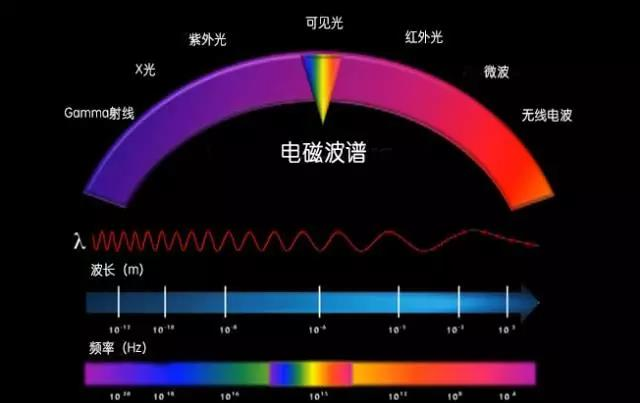
\includegraphics[width=0.70\textwidth]{figs/2021-12-02-16-23-16.png}
    \end{center}
    光只是一定波长范围内的电磁波
\end{frame}

\begin{frame} 
    波动说面临的困难:
    \begin{itemize}
        \Item  黑体辐射
        \Item  光电效应
        \Item  康普顿效应
        \Item  氢原子光谱
    \end{itemize}
\end{frame}

%%%%%%%%%%%%%%%%%%%%%%%%%%%%%%%%%%%%
\subsection{光电效应}
%%%%%%%%%%%%%%%%%%%%%%%%%%%%%%%%%%%%

\begin{frame} 
    \frametitle{光电效应实验}   
    \begin{center}
       \includegraphics[width=0.53\textwidth]{figs/2021-12-02-16-01-21.png}
   \end{center}  
   {\Bullet} 具有瞬时性 \\
   {\Bullet} 存在临界频率 $\nu_0$ \\
   {\Bullet} 光电子能量由光的频率决定
\end{frame}  

\begin{frame} 
    In 1905, Einstein considered the derivation of Planck's Law  \\
    \begin{itemize}
        \Item  Plank’s Law was consistent with experment but not with existing theory
        \Item  Rayleigh-Jeans Law was consistent with existing theory but not with experiment
        \Item  For treating Ultraviolet Catastrophe, he proposed the light quantum hypothesis
        \Item  Using light quantum hypothesis, he explained the Photoelectric effect
    \end{itemize}
\end{frame}

\begin{frame}
    \frametitle{}
        \begin{figure}
            \centering
            \subfigure[光强分布]{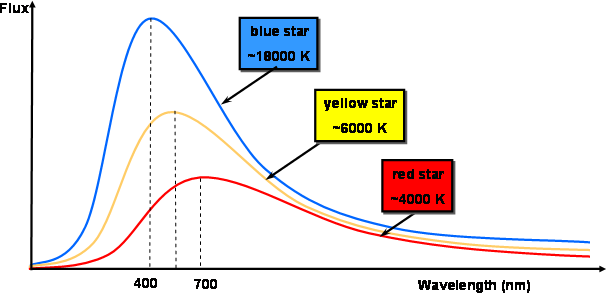
\includegraphics[width=0.495\textwidth]{figs/blackbody_radn_curves.png}}
            \subfigure[粒子数分布]{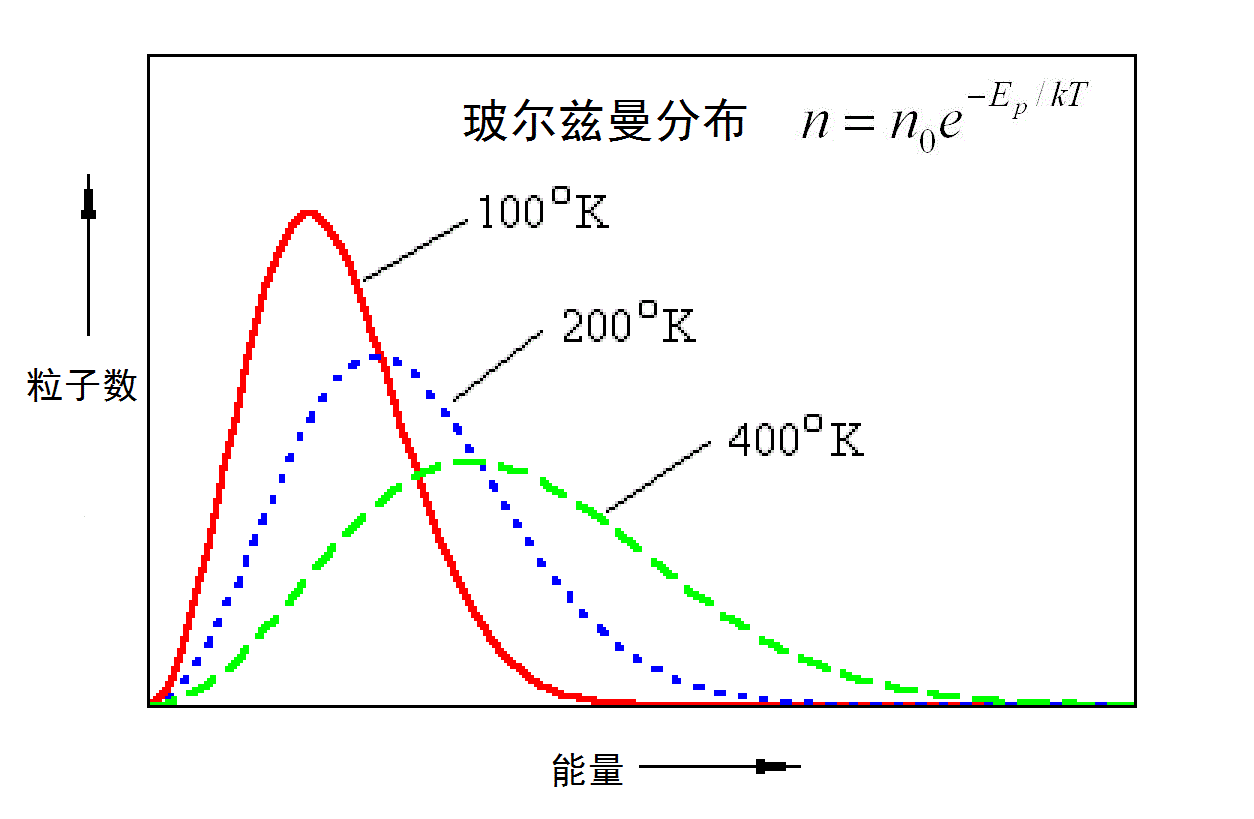
\includegraphics[width=0.495\textwidth]{figs/2022-01-17-14-21-43.png}}
        \end{figure}
    \setcounter{subfigure}{0}
\end{frame}

\begin{frame} 
    \begin{tcolorbox4}[Light quantum hypothesis]
        {\Bullet} Light likes particles with unit energy  (quanta).\\
        \[E=h\nu\]  
        {\Bullet} The energy of n light quantum is $nh\nu$. \\
        {\Bullet} The momentum of light quantum is (1918) \\
        \[p=\frac{E}{c}=\frac{h\nu}{c}=\frac{h}{\lambda}\]
    \end{tcolorbox4}
\end{frame}

\begin{frame} 
    基于光量子假说,提出光电效应公式
    \[
    \frac{1}{2}m_eV_0^2=h\nu-W
    \]
    \begin{itemize}
        \Item  瞬时性:光子碰上电子时,能量被瞬时吸收
        \Item  临界频率:$\nu_0=\frac{W}{h} $
        \Item  光电子能量与光的频率决定: $E_k=h\nu-W$
    \end{itemize}
    {\color{deepred} Nobel Prize in physics(1921)}
\end{frame}

\begin{frame} 
    基于光电效应公式:
$$
\frac{1}{2}m_eV_0^2=h\nu-W
$$
1916年,密立根实验上测定普朗克系数,验证光子说\\
\color{deepred}{1923年诺贝尔物理学奖} 
\end{frame}

\begin{frame} 
    \begin{tcolorbox4}[光量子假说的意义]
        \begin{itemize}
            \Item  揭示能量子的本质:在于光本身是量子化的,具有粒子性
            \Item  揭示光的本质:光既具波动性又具粒子性。
        \end{itemize}
    \end{tcolorbox4}
    \begin{quotation}
        "在近代物理学结出硕果的那些重大问题中,很难找到一个问题是爱因斯坦没有做出过重要贡献的。
        在他的各种推测中,他有时可能也曾经没有中标的,例如他的光量子假设,就有点迷失了方向\dots"  \\
        \rightline{$\cdots$ 普朗克\hspace{3em}}   
    \end{quotation}
\end{frame}

%%%%%%%%%%%%%%%%%%%%%%%%%%%
\subsection{康普顿效应}
%%%%%%%%%%%%%%%%%%%%%%%%%%%

\begin{frame}   
    \frametitle{康普顿效应 (1922)}
    \begin{center}
        \includegraphics[width=0.7\textwidth, height=3in]{figs/comptonscattering.png}
    \end{center}  
\end{frame}

\begin{frame} 
    ~~\\ 
    经验公式:$\lambda_{out}-\lambda_{in}=\lambda_e(1-\cos \theta)$ \\  \vspace*{0.6em}
    \alert{解:} Energy of electron 
    \begin{equation*}
        E^2 =m_ec^2=p^2c^2 +m_0 ^2 c^4 
    \end{equation*}
    Energy of light quantum
    \begin{equation*}
        E =pc 
    \end{equation*}
    energy conservation law
    \begin{equation*}
        \begin{split}
        E_i + m_0 c^2 &= E_o + m_ec^2 \\
        (E_i -E_o + m_0 c^2)^2 &= E_e ^2\\
        (p_i c-p_o c + m_0 c^2) ^2 &= p_e ^2 c^2 +m_0 ^2 c^4 \\
        (p_i-p_o)^2 +2 m_0 (p_i c-p_o c) &= p_e ^2
    \end{split}
    \end{equation*}
\end{frame}

\begin{frame}  
    momentum conservation law
    \begin{equation*}
        \begin{split}
            \vec{p}_i -\vec{p}_o &= \vec{p}_e \\
            (\vec{p}_i -\vec{p}_o)\cdot (\vec{p}_i -\vec{p}_o)  &= \vec{p}_e\cdot \vec{p}_e   \\
            p_i ^2 + p_o ^2 -2p_i p_o \cos \theta &= p_e ^2  \\
            p_i ^2 + p_o ^2 -2p_i p_o \cos \theta &= (p_i-p_o)^2 +2 m_0 (p_i c-p_o c) \\
            \frac{1}{p_o} -\frac{1}{p_i} &= \frac{1}{m_0 c} (1-\cos \theta) \\
            \lambda_o -\lambda_i &= \frac{h}{m_0 c} (1-\cos \theta) 
        \end{split}
    \end{equation*}
\end{frame}

\begin{frame}   
    \begin{tcolorbox3}[Significance]
        Prove that:\\
        {\Bullet} The light of wavelength ($\lambda$) possesses a quantum momentum \[p=\frac{h}{\lambda}\]
        {\Bullet} Momentum conservation law works in subatom scales 
    \end{tcolorbox3}   
    \color{deepred}{Nobel Prize in physics(1927)}\\
\end{frame}

%%%%%%%%%%%%%%%%%%%%%%%%%%
\subsection{氢原子光谱}
%%%%%%%%%%%%%%%%%%%%%%%%%%

\begin{frame}  
     \frametitle{氢原子光谱}
     \begin{center}
        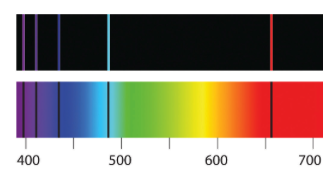
\includegraphics[width=0.6\textwidth]{figs/2022-01-17-14-02-45.png}
    \end{center}  
    经验公式:
       $\dfrac{1}{\lambda}=R_H c (\dfrac{1}{m^2} -\dfrac{1}{n^2})$ \\ \vspace{0.3em}
    \alert{Problem:} the formula cannot be derived from existing theory
\end{frame}

\begin{frame} 
    \frametitle{Rutherford model}  
    \begin{center}
        \includegraphics[width=0.8\textwidth]{figs/utherford_atom.png}
    \end{center}  
\end{frame}

\begin{frame}  
    \begin{tcolorbox4}[Bohr's hydrogen atom hypothesis]
    Bohr asummed that :\\
    {\Bullet} Stationary states: Electrons move around the nucleus only in certain allowed circular orbits with fixed energy \\
    \[ L=n \frac{h}{2\pi}= n \hbar,\qquad (\oint p_i dq_i = n_i h)\]
    {\Bullet} Quantum transition: Electron can jump between stationary state orbits when absorbed or emitted a photon with certain energy\\
    \[ h\nu=E_n -E_m \]
    \end{tcolorbox4}
\end{frame}

\begin{frame}   
    \frametitle{}
    推导光谱公式\\
    {\Bullet} Stationary state orbit radius:
    \begin{equation*}
        \begin{split}
            m\frac{v^2}{r}&=\frac{1}{4\pi\epsilon_0} \frac{e^2}{r^2} \\
            L=&mvr =n\hbar \\
            r_n&= n^2 (\frac{\epsilon_0 h^2}{m\pi e^2}) =n^2 r_1   
        \end{split} 
     \end{equation*}
     {\Bullet} Stationary state orbit energy: 
     \begin{equation*}
        \begin{split}
            E_n &= T + U \\
            &= \frac{1}{2}mv^2- \frac{1}{4\pi\epsilon_0} \frac{e^2}{r_n ^2} \\
            &= \frac{1}{n^2} (-\frac{m e^4}{8 \epsilon_0 ^2 h^2}) = \frac{E_1}{n^2}
        \end{split}  
     \end{equation*}
\end{frame}

\begin{frame}
    {\Bullet} Spectrum formula: 
    \begin{equation*}
        \begin{split}
         \nu&=\frac{E_n -E_m}{h} \\
         &= \frac{m e^4}{4\pi \hbar ^3} [\frac{1}{m^2} -\frac{1}{n^2}]
        \end{split}  
     \end{equation*}
     {\Bullet} Rydberg constant : 
     \[R_{theo}= \frac{m e^4}{4\pi \hbar ^3 c} =1.0973731\times 10^7 m^{-1}\]
    \[R_{exp}=1.0974\times10^7 m^{-1} \]  
\end{frame}

\begin{frame}   
    \frametitle{Bohr's model}  
    \begin{center}
        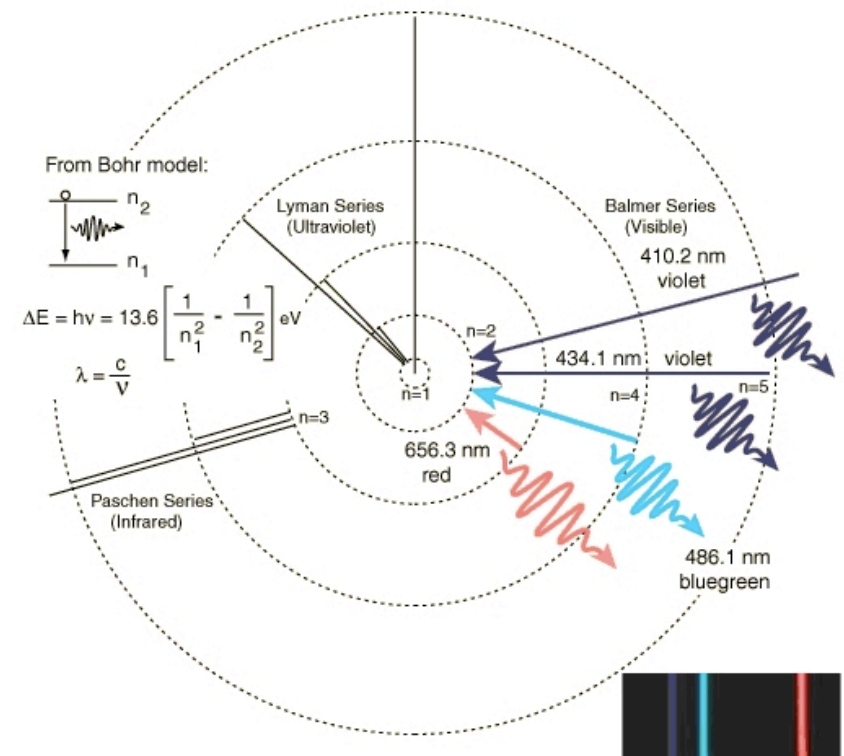
\includegraphics[width=0.6\textwidth]{figs/bohrmodel.png}
    \end{center}  
    {\Bullet} 1905年爱因斯坦提出的光子概念,不受名人的重视,普朗克把爱因斯坦的光量子概念说成是“迷失了方向”。\\
    {\Bullet} 1913年,28岁的玻尔,创造性地把光子概念用到卢瑟福模型上,成功破解氢原子光谱问题 \\
    {\color{deepred} {\Bullet} Nobel Prize in physics(1922)}\\ 
\end{frame}

\subsection{光的波粒二象性} 

\begin{frame} 
  \frametitle{光的波粒二象性}  
  {\Bullet} In 1905, when Einstein first put forward this hypothesis, 
  he simply stated that light consisted of quanta with energy \[ E = h\nu \] 
  {\Bullet} In 1917, he stated that the light quantum carried a momentum of  \[ p=\frac{h}{\lambda}\]
  At this point, the light quantum with massless particle property was named as photon (光子)
\end{frame}

\begin{frame}  
  $\begin{cases}
    \text{Light behaves like waves }\\
    \text{~~\qquad Interference} \\
    \text{~~\qquad Diffraction} \\
    \text{Light behaves like particles}\\
    \text{~~\qquad Black body radiation} \\
    \text{~~\qquad Photoelectric effect} \\
    \text{~~\qquad Compton effect} \\
   \end{cases}$\\
   ~~\\
   Light has both wave and particle properties is called \alert{wave-particle duality} of light
\end{frame}

\begin{frame}
    \frametitle{}
    \begin{tcolorbox3}[学术讨论]
        ~\\
        How can the light be both particle and wave ?
    \end{tcolorbox3}
\end{frame}

%%%%%%%%%%%%%%%%%%%%%%%%%%%
\subsection{物质波假说}
%%%%%%%%%%%%%%%%%%%%%%%%%%%

\begin{frame}   
  \frametitle{物质波假说}
  \begin{tcolorbox4}[Matter wave hypothesis]
  In 1923, de Broglie states that if light which is classically a wave could behave as a particle
  then classical particles could also behave as quantum waves. The wave length and frequency are
  \[\lambda=\frac{h}{p}\]
  \[\nu =\frac{E}{h}\]
  \end{tcolorbox4}
\end{frame}

\begin{frame}  
    \frame{}
    Calculating de Broglie wavelength of electron in Bohr's H atom model
    \begin{equation*}
        \begin{split}
            L&=n\hbar \\
            \vec{r} \cdot \vec{p} & =  n\frac{h}{2 \pi} \\
            2\pi r&=  n\frac{h}{p}\\
            2\pi r&=  n\lambda 
        \end{split} 
     \end{equation*}
     Now, we called it standing-wave condition 
\end{frame}


\begin{frame}   
  \frametitle{Experimental verification}
  \begin{center}
    \includegraphics[width=0.5\textwidth]{figs/elediffr.jpeg} \\
    Electron diffraction patterns (Davisson and Germer, 1927)
    \end{center} 
\end{frame}
\begin{frame}   
    \begin{center}
      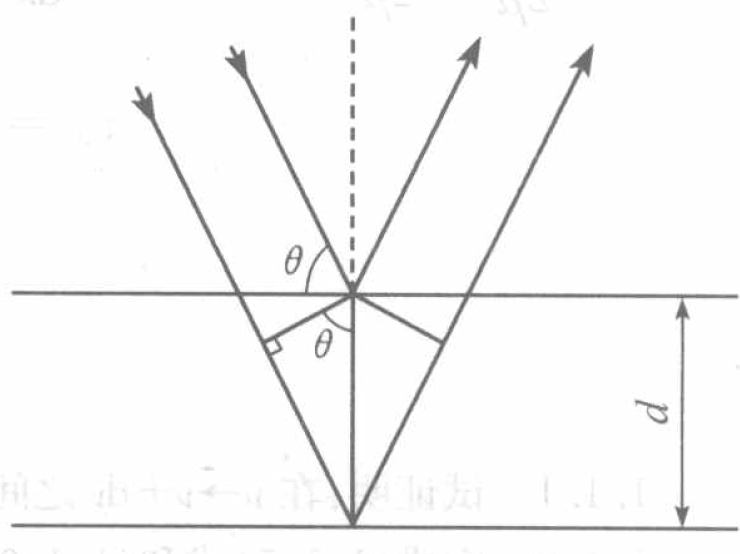
\includegraphics[width=0.55\textwidth]{figs/scatting.png} \\
    \end{center} 
    \begin{itemize}
        \Item  Meeting Bragg formula $2d\sin \theta=n\lambda $
        \Item  Obtaining the wavelength of electron (about 0.16X $nm$), agreeing well with the 
   calculated de Broglie wavelength 
    \end{itemize}
  {\color{deepred} Nobel Prize in physics(1937)}  
  \end{frame}

  \begin{frame}
      \frametitle{}
    \begin{center}
         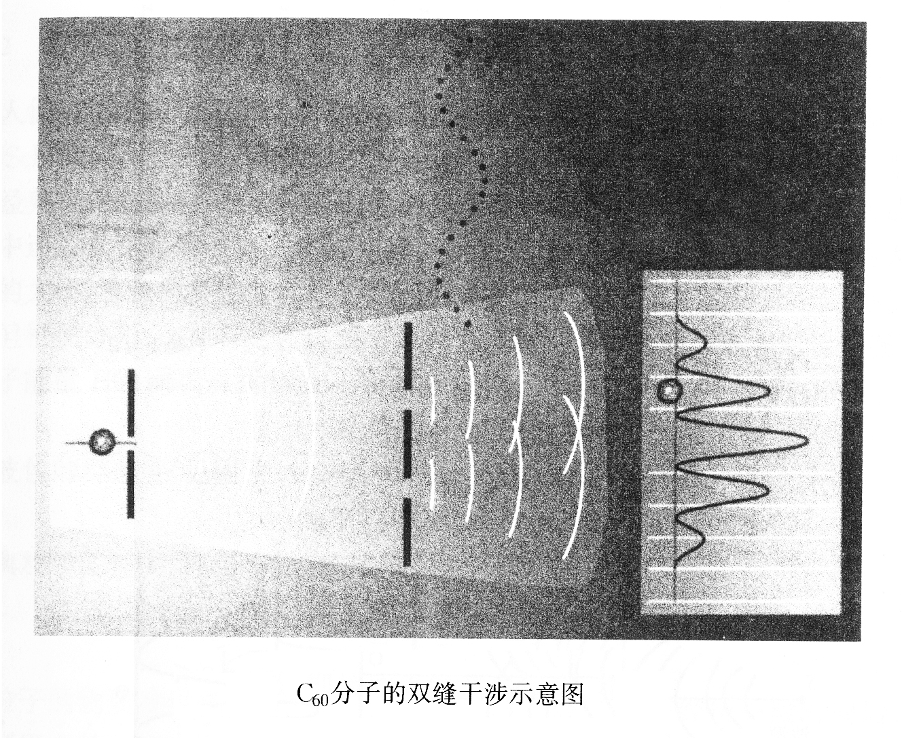
\includegraphics[width=0.8\textwidth,height=2.5in]{figs/c60.png}
    \end{center}
  \end{frame}
\begin{frame} 
    \begin{tcolorbox}[colback=yellow!10,colframe=red!75!black,title=Significance]
        De Broglie extended the wave-particle duality from light to particles! \\
        {\color{deepred} Nobel Prize in physics(1929)} for discovery of wave nature of electrons
    \end{tcolorbox}  
\end{frame}

\begin{frame}{电子双缝干涉实验}
    \includemedia[
    width=1.0\linewidth,height=0.67\linewidth, % 16:9
    activate=pageopen,
    addresource=figs/doubleslite-n.mp4,
    flashvars={
    source=figs/doubleslite-n.mp4
    &autoPlay=true % start playing on activation
    &loop=true
    }
    ]{}{VPlayer.swf}
\end{frame}

\begin{frame}
    \frametitle{学术讨论}
        \begin{figure}
            \centering
            \subfigure[]{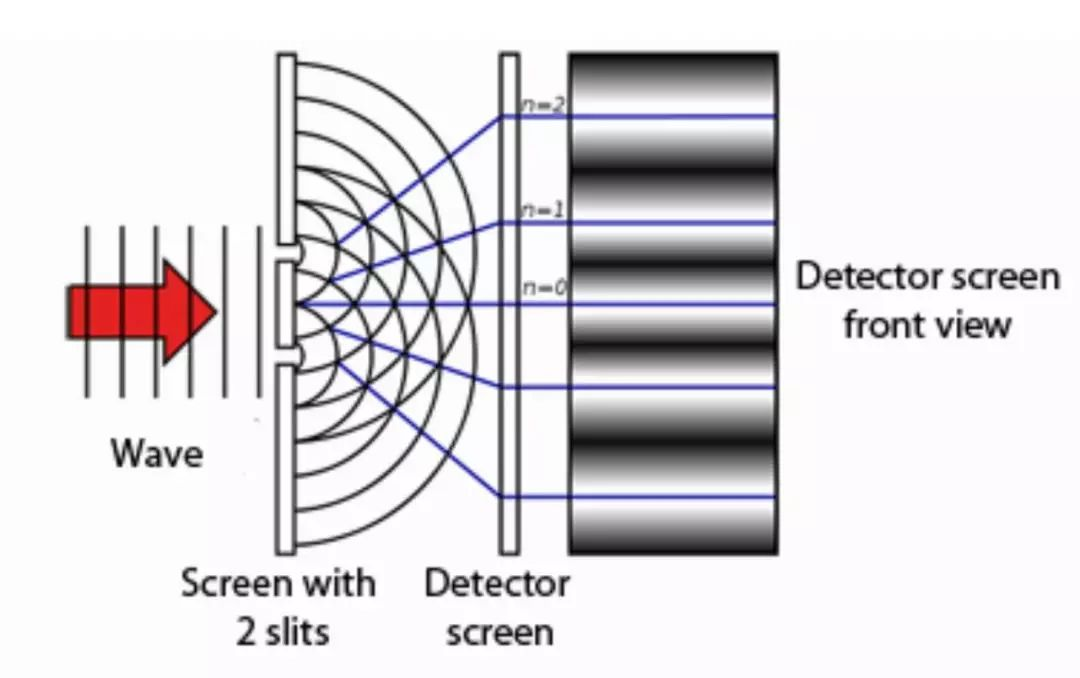
\includegraphics[width=4.5cm]{figs/ds-1.jpeg}}
            \subfigure[]{\includegraphics[width=4.5cm]{figs/ds-2.jpeg}}
            \subfigure[]{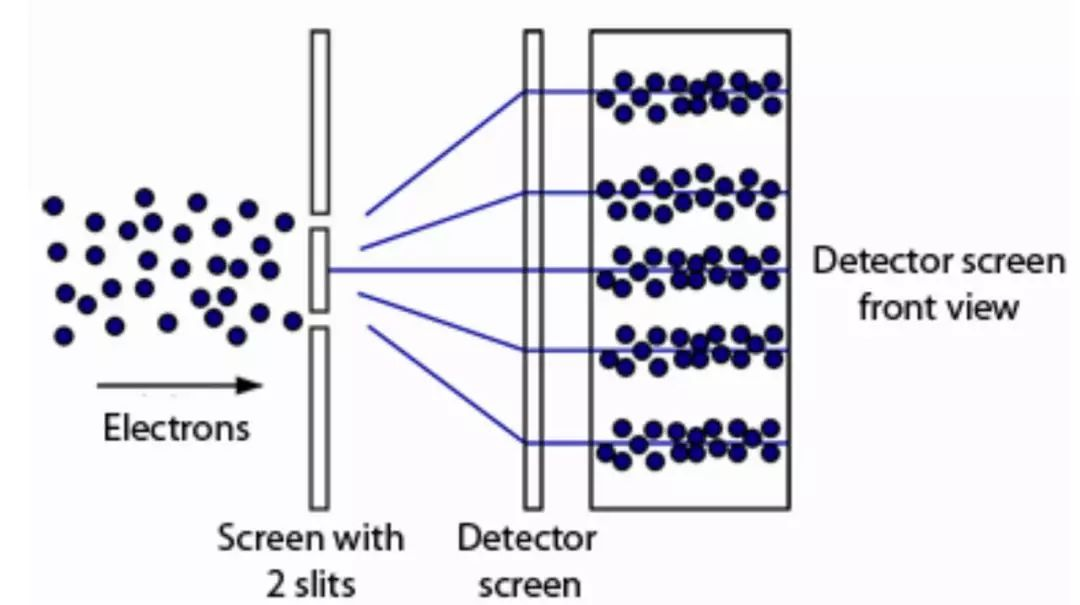
\includegraphics[width=4.5cm]{figs/ds-3.jpeg}}
            %\caption{} %图片标题
            %\label{fig:1}  
            {\color{red} How can electrons be both a particle and a wave?}
        \end{figure}
    \setcounter{subfigure}{0}
\end{frame}

\begin{frame}  
    \begin{tcolorbox3}[Conclusion]
    Wave-particle duality is the inherent attribute of matter
    \end{tcolorbox3} 
\end{frame} 

\begin{frame}
    \frametitle{}
    \centering
    \tcbb[0.5]{Big problems}
    {
      \large  How to interpret a world where waves are particles and particles are waves
    }
\end{frame}

%%%%%%%%%%%%%%%%%%%%%%%%%%%%%%%%%%%%%%%%%%%%%%%%%%%%%%%%%%%%%%%%%%%
\begin{frame}
    \frametitle{课外作业}
    \begin{enumerate}
        \item 计算氢原子第一玻尔半径上电子的德布罗意波长
        \item 计算经 50 V 电势装成加速后电子的德布罗意波长
    \end{enumerate}
\end{frame}
%%%%%%%%%%%%%%%%%%%%%%%%%%%%%%%%%%%%%%%%%%%%%%%%%%%%%%%%%%%%%%%%%%%